
\subsubsection{Yocto ou Buildroot, comment choisir ?}
\paragraph{}
Yocto est donc très adapté pour une image nécessitant une multitude de dépendances externes, pour un développement court et focalisé sur les fonctionnalités propres du produit, avec une gamme de produits proposant des fonctionnalités légèrement différentes. Yocto permet de factoriser le développement et de rendre modulable l'OS embarqué.  Buildroot est, quant à lui, plus adapté à des projets plus modestes, où la mise à jour est moins fréquente. Buildroot crée des OS statiques, adaptés aux outils plus bas niveau, peut être moins évolués, se focalisants sur la robustesse. Buildroot est également plus simple à prendre en main, ce qui est un atout non négligeable. Il sera en revanche moins adapté au travail en groupe. 


\begin{figure}[ht!] 
\begin{center}
    

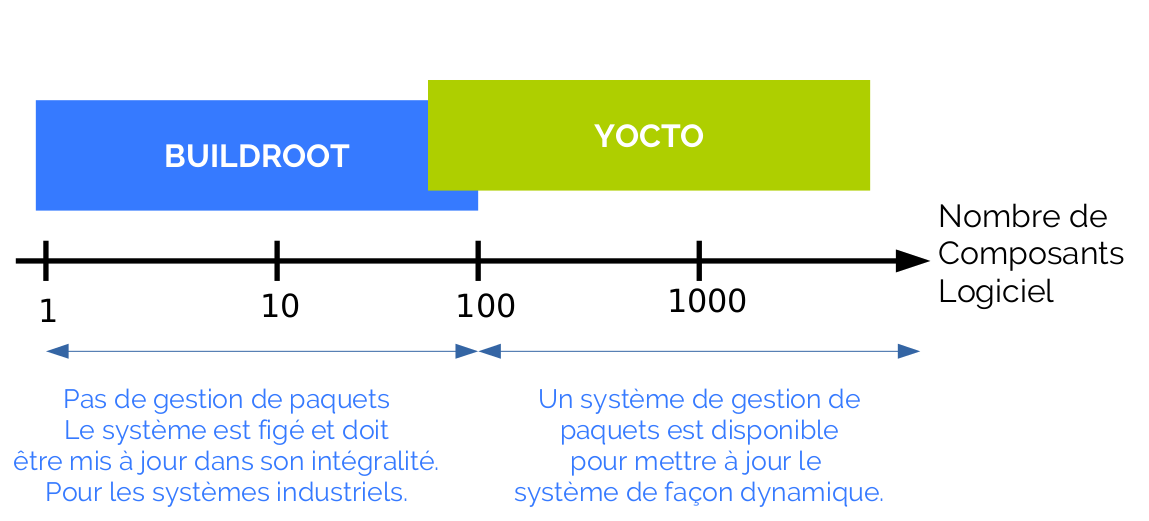
\includegraphics[width=13cm]{Images/yocto comp log.png} % Figure image 

\caption{crédit: Yocto project} % Figure caption 

\end{center}
\label{Project Yocto} % Label for referencing with \ref{bear} 
\end{figure}

On peut donc résumer : 
Le projet
\begin{itemize}

\item comporte une gamme de produit - Yocto facilitera la factorisation du développement
\item comporte de nombreux modules externe - Yocto
\item repose sur des ajouts de fonctionnalité fréquentes - Yocto
\item est un système figé, un code métier peu évolutif et peu de composants externe - Buildroot fera très bien l'affaire
\end{itemize}

Tout ce que peut faire Buildroot, Yocto en est également capable. Le passage de Buildroot à Yocto est pertinent si le projet est important, qu'il doit être porté sur différentes plateformes et qu'il nécessite de nombreuses composantes de la communauté. Si la composante centrale du projet n'est pas logiciel, que tout repose sur le code métier, avec un cycle de développement long, Buildroot est adapté et une évolution n'est pas forcément pertinente.